\documentclass[border=10pt]{standalone}
\usepackage{tikz}
\usetikzlibrary{arrows.meta}

\begin{document}
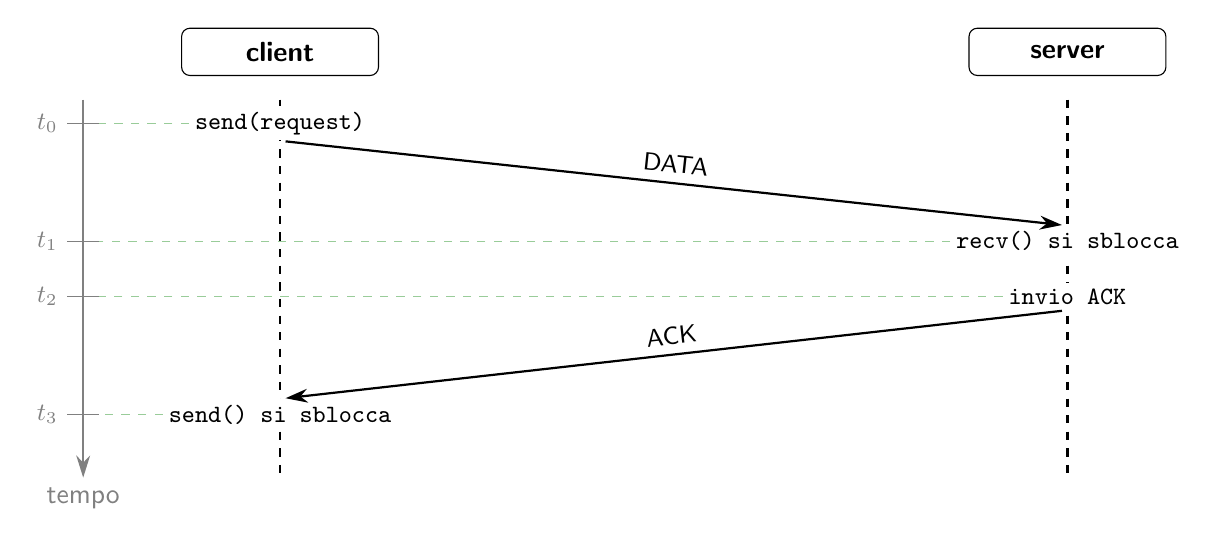
\begin{tikzpicture}[
    >={Stealth[length=8pt, width=5pt]},
    msg/.style={->, thick, shorten >=2pt, shorten <=2pt},
    event/.style={font=\small\ttfamily, fill=white, inner sep=2pt},
    label/.style={font=\small\sffamily, midway, above, sloped}
  ]

  % Asse del tempo
  \draw[->, gray, thick] (-2.5, 0.3) -- (-2.5, -4.5) node[below, font=\sffamily] {tempo};
  \foreach \y/\t in {0/t_0, -1.5/t_1, -2.2/t_2, -3.7/t_3} {
    \draw[gray] (-2.7, \y) -- (-2.3, \y);
    \node[left, font=\small\sffamily, gray] at (-2.7, \y) {$\t$};
  }

  % Linee di vita
  \draw[thick, dashed] (0, 0.3) -- (0, -4.5);
  \draw[thick, dashed] (10, 0.3) -- (10, -4.5);

  % Intestazioni
  \node[above, font=\bfseries\sffamily, fill=white, draw, rounded corners=3pt, minimum width=2.5cm, minimum height=0.6cm] (hclient) at (0, 0.6) {client};
  \node[above, font=\bfseries\sffamily, fill=white, draw, rounded corners=3pt, minimum width=2.5cm, minimum height=0.6cm] (hserver) at (10, 0.6) {server};

  % Eventi
  \node[event] (send)    at (0,  0)    {send(request)};
  \node[event] (recv)    at (10, -1.5) {recv() si sblocca};
  \node[event] (ack)     at (10, -2.2) {invio ACK};
  \node[event] (sendok)  at (0,  -3.7) {send() si sblocca};

  % Linee guida evento -> tick temporale
  \draw[green!50!black, opacity=0.4, thin, dashed] (send.west)   -- (-2.3, 0);
  \draw[green!50!black, opacity=0.4, thin, dashed] (recv.west)   -- (-2.3, -1.5);
  \draw[green!50!black, opacity=0.4, thin, dashed] (ack.west)    -- (-2.3, -2.2);
  \draw[green!50!black, opacity=0.4, thin, dashed] (sendok.west) -- (-2.3, -3.7);

  % Frecce
  \draw[msg] (send.south)  -- node[label] {DATA} (recv.north);
  \draw[msg] (ack.south)   -- node[label] {ACK}  (sendok.north);

\end{tikzpicture}
\end{document}
